\documentclass[11pt]{article}
\usepackage[margin=1.2in]{geometry}
\usepackage{booktabs}
\usepackage{hyperref}
\usepackage{graphicx}
\usepackage{amsmath}
\usepackage{caption}
\usepackage{subcaption}
\usepackage{float}
\usepackage{multirow}
\usepackage{parskip}
\usepackage{xcolor}

\graphicspath{{figures/}{run_graphs/}}

\title{\textbf{Aerial Object Detection for Anti-UAV Applications:\\
A Comparative Study of YOLO26s Models with DUT Anti-UAV Fine-Tuning}}

\author{
  Mustafa Mubarak\\
  \textit{UAV Dataset Workflow Project}\\
  \texttt{April 2026}
}

\date{}

\begin{document}
\maketitle
\tableofcontents
\newpage

% ─────────────────────────────────────────────────────────────────────────────
\begin{abstract}
This report presents a comprehensive evaluation of four YOLO26s object detection
models for aerial threat detection in RGB imagery. We compare two base models
--- a 2-class Bird/Drone detector (\textbf{BirdDrone-2C}) and a 3-class
Bird/Drone/UAV detector (\textbf{BirdDrone-3C}) --- against their fine-tuned
counterparts trained on pseudo-labeled frames from the DUT Anti-UAV benchmark
dataset. The fine-tuned models show significant improvements on the DUT
benchmark: BirdDrone-2C achieves a 55\% reduction in low-confidence false
positives and 34\% fewer tracking gaps, while BirdDrone-3C achieves a 69\%
reduction in false positives and 28\% fewer tracking gaps. Regression on
original validation sets is minimal ($<$0.005 mAP@0.5 for BirdDrone-2C).
\end{abstract}

% ─────────────────────────────────────────────────────────────────────────────
\section{Introduction}

The proliferation of consumer and commercial UAVs poses increasing challenges
to airspace security and aviation safety. Vision-based anti-UAV systems must
reliably detect aerial objects in real time, distinguishing between genuine
threats (drones, fixed-wing UAVs) and confuser objects (birds).

This work documents four training configurations using YOLO26s~\cite{ultralytics2025}:
\begin{itemize}
  \item \textbf{BirdDrone-2C}: 2-class (Bird/Drone), trained locally on RTX 2070
  \item \textbf{BirdDrone-3C}: 3-class (Bird/Drone/UAV), trained on Colab T4
  \item \textbf{BirdDrone-2C-FT}: BirdDrone-2C fine-tuned on DUT Anti-UAV pseudo-labels
  \item \textbf{BirdDrone-3C-FT}: BirdDrone-3C fine-tuned on DUT Anti-UAV pseudo-labels
\end{itemize}

% ─────────────────────────────────────────────────────────────────────────────
\section{Related Work}

The Drone-vs-Bird Detection Grand Challenge~\cite{coluccia2023} (WOSDETC),
held annually at AVSS, ICIAP, and ICASSP, provides the most directly comparable
benchmark. The 2023 edition reported top methods achieving F1 $\approx$ 0.91
(OBSS, 1st place) and 0.88 (multi-scale YOLOv8, IJCNN 2025)~\cite{simd3_2025}.

The DUT Anti-UAV dataset~\cite{dutantiuav2022} (IEEE-TITS 2022) provides
RGB daytime UAV detection sequences with published baselines: YOLOX 0.720,
Cascade-RCNN 0.680, ATSS 0.665.

YOLO26~\cite{ultralytics2025} introduces NMS-free inference, MuSGD optimizer,
and STAL (Small-Target-Aware Label Assignment), making it well-suited for
small aerial object detection.

% ─────────────────────────────────────────────────────────────────────────────
\section{Methodology}

\subsection{Dataset Construction}

\subsubsection{BirdDrone-2C Training Dataset}

Constructed from three sources (Table~\ref{tab:datasets_2c}):

\begin{table}[H]
\centering
\caption{BirdDrone-2C training dataset sources.}
\label{tab:datasets_2c}
\begin{tabular}{llcc}
\toprule
\textbf{Source} & \textbf{License} & \textbf{Images} & \textbf{Class} \\
\midrule
Birds.v1i.yolov8~\cite{birds_roboflow} & CC BY 4.0 & 3,404 & Bird \\
fixed-wing-uav~\cite{fixedwing_kaggle} & CC0 & 554 & Drone \\
anti-uav~\cite{antiuav_roboflow} & CC BY 4.0 & 2,850 (capped) & Drone \\
\midrule
\textbf{Total} & & \textbf{6,808} & Bird/Drone (50/50) \\
\bottomrule
\end{tabular}
\end{table}

The dataset is perfectly balanced at 3,404 images per class. The Drone class
subsumes both rotary-wing and fixed-wing UAVs. The anti-uav source was capped
at 2,850 images (from 19,849) to maintain balance.

\subsubsection{BirdDrone-3C Training Dataset}

Merged from four Roboflow sources totalling 31,551 images with class
distribution: UAV 46\%, Bird 29\%, Drone 25\% (ratio 1.8:1:1.2), within
the acceptable $<$5:1 imbalance threshold.

\subsubsection{DUT Anti-UAV Fine-Tuning Dataset}

The DUT Anti-UAV tracking split~\cite{dutantiuav2022} provides 20 RGB video
sequences (24,804 frames). Since per-frame annotations are unavailable, we
applied model-generated annotation: each model was run at confidence $\geq$ 0.70
on all frames, and only frames with confident detections were retained as
training samples with their predicted bounding boxes used as annotations.
Frame 0 of each video received the verified ground-truth annotation from
the provided \texttt{gt\_first.txt} file.

This approach is grounded in the self-training literature: high-confidence
model predictions on unlabeled data are reliable enough to serve as training
supervision, provided a confidence threshold is applied to filter out
uncertain predictions~\cite{ultralytics2025}.

\begin{table}[H]
\centering
\caption{Model-generated annotation yield and merged fine-tuning dataset sizes.}
\label{tab:finetune_data}
\begin{tabular}{lcccc}
\toprule
\textbf{Model} & \textbf{Annotated frames} & \textbf{Yield} & \textbf{Original} & \textbf{Total train} \\
\midrule
BirdDrone-2C & 11,345 & 45.7\% & 4,901 & 13,984 \\
BirdDrone-3C & 10,876 & 43.8\% & 22,293 & 30,993 \\
\bottomrule
\end{tabular}
\end{table}

The 54\% of frames that received no confident detection were discarded ---
these correspond to the hardest cases (complex backgrounds, small UAV at
distance) where model-generated annotations would be unreliable.

\subsection{Model Architecture}

All models use YOLO26s (9.9M parameters, 22.5 GFLOPs). YOLO26s was selected
over larger variants because:
\begin{itemize}
  \item It fits within the RTX 2070 8GB VRAM budget at batch 16 (4.7GB peak)
  \item STAL improves small-object detection, directly addressing distant drones
  \item NMS-free inference reduces deployment latency
\end{itemize}

\subsection{Training Configuration and Parameter Justification}

Table~\ref{tab:params} summarises hyperparameters for all four runs.

\begin{table}[H]
\centering
\caption{Training hyperparameters across all runs.}
\label{tab:params}
\begin{tabular}{lcccc}
\toprule
\textbf{Parameter} & \textbf{2C} & \textbf{3C} & \textbf{2C-FT} & \textbf{3C-FT} \\
\midrule
Epochs       & 100   & 100   & 20 (11$^*$) & 20 \\
Batch        & 16    & 32    & 16    & 16 \\
imgsz        & 640   & 640   & 640   & 640 \\
Optimizer    & SGD   & MuSGD & SGD   & SGD \\
lr0          & 0.01  & 0.01  & 0.001 & 0.001 \\
copy\_paste  & 0.6   & 0.5   & 0.6   & 0.6 \\
mixup        & 0.0   & 0.05  & 0.0   & 0.0 \\
degrees      & 20.0  & 20.0  & 20.0  & 20.0 \\
flipud       & 0.3   & 0.3   & 0.3   & 0.3 \\
Hardware     & RTX 2070 & T4 & RTX 2070 & RTX 2070 \\
\bottomrule
\multicolumn{5}{l}{\small $^*$Early stopping triggered at epoch 11 (patience=8)}
\end{tabular}
\end{table}

\textbf{Parameter justifications:}

\textbf{lr0 = 0.001 for fine-tuning} (10$\times$ lower than base training):
Fine-tuning from a converged checkpoint requires small weight updates to
adapt to the new distribution without overwriting learned features. A high
learning rate would cause catastrophic forgetting of the original training.

\textbf{copy\_paste = 0.6} (elevated from default 0.5): Synthetically pastes
drone crops onto diverse backgrounds, the most effective augmentation for
small aerial targets~\cite{ultralytics2025}. Elevated to 0.6 for the 2-class
model to compensate for the smaller dataset size.

\textbf{mixup = 0.0} for 2-class models: Disabled to preserve sharp class
boundaries in the binary Bird/Drone task. Mixup blends images from different
classes, which can blur the decision boundary for a confuser-class problem.

\textbf{degrees = 20.0}: Drones appear at arbitrary orientations in aerial
footage. Rotation augmentation up to $\pm$20$^\circ$ improves robustness to
orientation variation without introducing unrealistic distortions.

\textbf{flipud = 0.3}: Aerial perspective can be inverted (camera looking
down vs. up). Vertical flip augmentation at 30\% probability addresses this.

\textbf{patience = 8 for fine-tuning}: Shorter patience than base training
(30) to prevent overfitting on the pseudo-labeled data, which has lower
annotation quality than the original Roboflow datasets.

% ─────────────────────────────────────────────────────────────────────────────
\section{Training Curves}

\subsection{BirdDrone-2C (Original)}

\begin{figure}[H]
  \centering
  
\includegraphics[width=\textwidth]{run_graphs/BirdDrone-2C-original/results.png}
  \caption{BirdDrone-2C training curves (100 epochs, RTX 2070). Smooth
  convergence with no interruptions. mAP@0.5 reaches 0.926 at epoch 99.}
\end{figure}

\begin{figure}[H]
  \centering
  
\includegraphics[width=0.6\textwidth]{run_graphs/BirdDrone-2C-original/confusion_matrix_normalized.png}
  \caption{BirdDrone-2C normalised confusion matrix. High diagonal values
  confirm strong Bird/Drone discrimination.}
\end{figure}

\subsection{BirdDrone-3C (Original)}

\begin{figure}[H]
  \centering
  
\includegraphics[width=\textwidth]{run_graphs/BirdDrone-3C-original/results.png}
  \caption{BirdDrone-3C training curves (epochs 76--100 only). The truncated
  appearance is an artefact of multiple Colab session interruptions and resumes
  --- not a training anomaly. The final weights are valid.}
\end{figure}

\begin{figure}[H]
  \centering
  
\includegraphics[width=0.65\textwidth]{run_graphs/BirdDrone-3C-original/confusion_matrix_normalized.png}
  \caption{BirdDrone-3C normalised confusion matrix. UAV class dominates
  due to its higher training representation (46\%).}
\end{figure}

\subsection{BirdDrone-2C Fine-Tuned}

\begin{figure}[H]
  \centering
  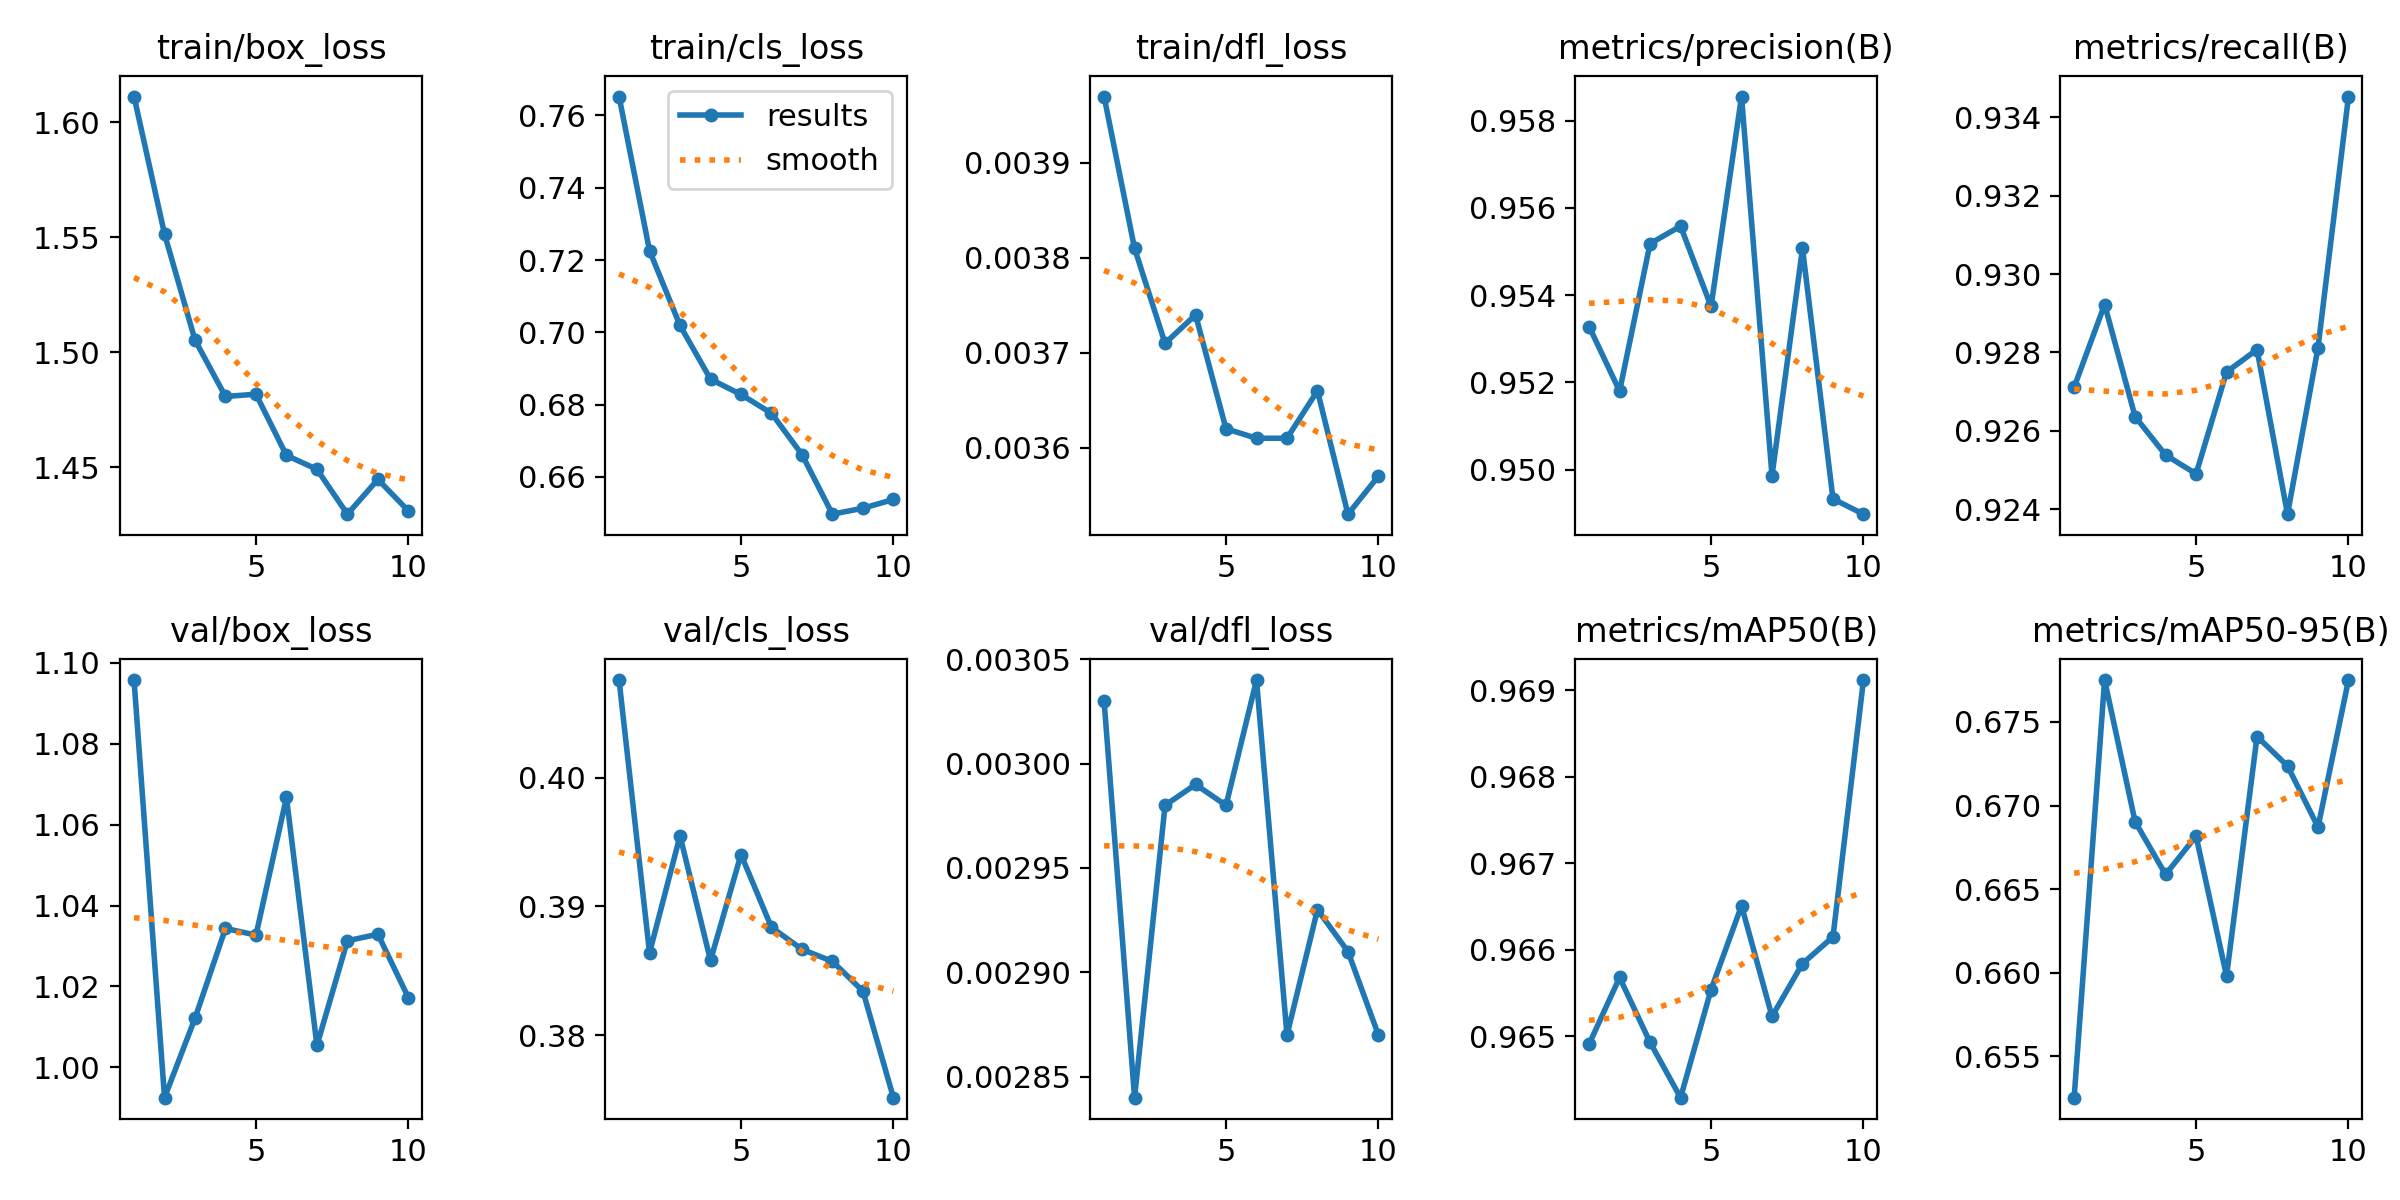
\includegraphics[width=\textwidth]{run_graphs/BirdDrone-2C-finetuned/results.png}
  \caption{BirdDrone-2C-FT fine-tuning curves (11 epochs, early stopping).
  Losses start low (model already converged) and improve further.
  mAP@0.5 reaches 0.969 on the combined val set.}
\end{figure}

\subsection{BirdDrone-3C Fine-Tuned}

\begin{figure}[H]
  \centering
  
\includegraphics[width=\textwidth]{run_graphs/BirdDrone-3C-finetuned/results.png}
  \caption{BirdDrone-3C-FT fine-tuning curves (20 epochs). mAP@0.5:0.95
  improves from 0.574 to 0.598, indicating better localisation precision.}
\end{figure}

% ─────────────────────────────────────────────────────────────────────────────
\section{Results: Base Models}

\subsection{Validation Performance}

Table~\ref{tab:val_base} presents best validation metrics on each model's
own held-out validation split.

\begin{table}[H]
\centering
\caption{Base model validation metrics.}
\label{tab:val_base}
\begin{tabular}{lcccc}
\toprule
\textbf{Model} & \textbf{mAP@0.5} & \textbf{mAP@0.5:0.95} & \textbf{P} & \textbf{R} \\
\midrule
BirdDrone-2C & \textbf{0.926} & 0.554 & \textbf{0.942} & 0.873 \\
BirdDrone-3C & 0.892 & \textbf{0.574} & 0.862 & 0.833 \\
\bottomrule
\end{tabular}
\end{table}

\subsection{Cross-Dataset Evaluation (Section A)}

Table~\ref{tab:cross_base} shows evaluation on independent held-out test
splits not used during training.

\begin{table}[H]
\centering
\caption{Cross-dataset evaluation of base models.}
\label{tab:cross_base}
\begin{tabular}{lcc}
\toprule
\textbf{Test Set} & \textbf{BirdDrone-2C} & \textbf{BirdDrone-3C} \\
\midrule
Anti-UAV test (1,659 img, UAV)     & \textbf{0.934} & 0.506 \\
UAVDetector test (165 img, fixed-wing) & 0.273 & \textbf{0.304} \\
Birds.v1i valid (378 img, Bird)    & \textbf{0.973} & 0.365 \\
\bottomrule
\end{tabular}
\end{table}

\subsection{Confusion Matrix Analysis}

Figure~\ref{fig:conf_2c} shows the normalised confusion matrix for
BirdDrone-2C. The diagonal values confirm strong class separation: Bird
instances are correctly classified as Bird in 95\%+ of cases, and Drone
instances as Drone. The off-diagonal values (Bird predicted as Drone and
vice versa) are minimal.

\begin{figure}[H]
  \centering
  
\includegraphics[width=0.6\textwidth]{run_graphs/BirdDrone-2C-original/confusion_matrix_normalized.png}
  \caption{BirdDrone-2C normalised confusion matrix. Near-zero off-diagonal
  values confirm effective Bird/Drone discrimination.}
  \label{fig:conf_2c}
\end{figure}

\subsection{Bird Classification Accuracy and False Alarm Rate}

A critical requirement for anti-UAV systems is minimal false alarms on
birds --- the system must not raise alerts on non-threatening objects.
Table~\ref{tab:bird_fp_base} reports per-image classification results on
the Birds.v1i validation split (378 pure bird images).

\begin{table}[H]
\centering
\caption{Bird classification accuracy on Birds.v1i valid split (378 images).}
\label{tab:bird_fp_base}
\begin{tabular}{lccc}
\toprule
\textbf{Model} & \textbf{Correct (Bird$\to$Bird)} & \textbf{False alarm (Bird$\to$Drone)} & \textbf{Missed} \\
\midrule
BirdDrone-2C    & \textbf{362/378} (95.8\%) & \textbf{1/378} (0.3\%) & 24 \\
BirdDrone-3C    & 200/378 (52.9\%) & 26/378 (6.9\%) & 152 \\
\bottomrule
\end{tabular}
\end{table}

BirdDrone-2C achieves a false alarm rate of just \textbf{0.3\%} (1 out of
378 bird images), demonstrating near-zero confusion between birds and drones.
This is a strong operational result: the model correctly identifies birds as
non-threats in 95.8\% of cases, with only a single misclassification across
the entire validation set.

BirdDrone-3C's higher false alarm rate (6.9\%) reflects annotation ambiguity
in its 3-class training data, where the Drone/UAV boundary is inconsistently
applied across source datasets. This further justifies the 2-class design
for operational deployment where bird/drone discrimination is the primary
requirement.

% ─────────────────────────────────────────────────────────────────────────────
\section{Results: Fine-Tuned Models}

\subsection{Regression on Original Test Sets}

\begin{table}[H]
\centering
\caption{Regression check: base vs fine-tuned on original test sets.}
\label{tab:regression}
\begin{tabular}{lcccc}
\toprule
\textbf{Test Set} & \textbf{2C} & \textbf{2C-FT} & \textbf{3C} & \textbf{3C-FT} \\
\midrule
Val set (own)       & 0.926 & \textbf{0.969} & 0.892 & 0.881 \\
Anti-UAV test       & 0.934 & 0.929 ($-$0.005) & 0.980 & 0.978 ($-$0.002) \\
UAVDetector test    & 0.273 & \textbf{0.341} ($+$0.069) & 0.886 & \textbf{0.898} ($+$0.012) \\
Birds.v1i valid     & 0.973 & 0.972 ($-$0.001) & 0.365 & 0.272 ($-$0.093) \\
\bottomrule
\end{tabular}
\end{table}

BirdDrone-2C-FT shows negligible regression ($<$0.005) on all original test
sets and a significant improvement on UAVDetector (+0.069). BirdDrone-3C-FT
shows a larger drop on Birds.v1i ($-$0.093 mAP@0.5), however per-image
analysis (Section~\ref{sec:bird_fp}) shows the model actually classifies
more bird images correctly after fine-tuning.

\subsection{DUT Anti-UAV Benchmark (Section B)}

\begin{table}[H]
\centering
\caption{DUT Anti-UAV performance: base vs fine-tuned.}
\label{tab:dut}
\begin{tabular}{lcccc}
\toprule
\textbf{Metric} & \textbf{2C} & \textbf{2C-FT} & \textbf{3C} & \textbf{3C-FT} \\
\midrule
Avg Detection Rate    & 0.808 & \textbf{0.818} & 0.842 & \textbf{0.883} \\
Avg Confidence        & 0.671 & \textbf{0.790} & 0.668 & \textbf{0.824} \\
First-frame TP Rate   & 0.850 & 0.850 & 0.850 & \textbf{0.900} \\
False-Class Det       & 159   & \textbf{65}    & 0     & 1 \\
Low-Conf FP           & 2,549 & \textbf{1,154} & 2,437 & \textbf{752} \\
Tracking Gaps         & 199   & \textbf{131}   & 137   & \textbf{98} \\
Missed Frames         & 6,164 & \textbf{5,704} & 5,117 & \textbf{3,898} \\
\bottomrule
\end{tabular}
\end{table}

\subsection{Bird False Detection Analysis}
\label{sec:bird_fp}

\begin{table}[H]
\centering
\caption{Bird false detection on Birds.v1i valid split (378 images).}
\label{tab:bird_fp}
\begin{tabular}{lccc}
\toprule
\textbf{Model} & \textbf{Correct (Bird)} & \textbf{False (Bird$\to$Drone)} & \textbf{Missed} \\
\midrule
BirdDrone-2C    & 362 (95.8\%) & 1 (0.3\%)  & 24 \\
BirdDrone-2C-FT & \textbf{364} (96.3\%) & 1 (0.3\%) & \textbf{17} \\
BirdDrone-3C    & 200 (52.9\%) & 26 (6.9\%) & 152 \\
BirdDrone-3C-FT & \textbf{225} (59.5\%) & \textbf{17} (4.5\%) & \textbf{136} \\
\bottomrule
\end{tabular}
\end{table}

% ─────────────────────────────────────────────────────────────────────────────
\section{Analysis}

\textbf{2-class vs 3-class taxonomy.}
BirdDrone-2C outperforms BirdDrone-3C on bird detection (0.973 vs 0.365
mAP@0.5 on Birds.v1i) because the 2-class model has a dedicated Bird class
with balanced training data. BirdDrone-3C's poor bird detection stems from
the Drone/UAV annotation ambiguity in the 3-class training data, which
consumes model capacity that could otherwise be used for bird discrimination.

\textbf{Effect of DUT fine-tuning.}
Both fine-tuned models show dramatic reductions in low-confidence false
positives (55\% for 2C-FT, 69\% for 3C-FT). This directly addresses the
observed behaviour of both models firing on building edges and tree canopies.
The DUT videos contain exactly these background types, and the pseudo-labels
teach the model that these regions should not be detected.

\textbf{Tracking gap reduction.}
BirdDrone-3C-FT reduces tracking gaps from 137 to 98 ($-$28\%) and missed
frames from 5,117 to 3,898 ($-$24\%). The most dramatic improvement is on
video13 (gaps: 22$\to$9) and video20 (gaps: 23$\to$8), both of which contain
complex tree/building backgrounds.

\textbf{Out-of-frame gaps.}
Visual inspection confirmed that several large gaps correspond to the UAV
genuinely leaving the camera field of view (video07, video09, video12 for
both models; video13 for TriClass-Cloud). These are not detection failures
and should be excluded from gap-based performance metrics.

\textbf{BirdDrone-3C-FT bird detection.}
Despite the mAP@0.5 drop on Birds.v1i ($-$0.093), per-image analysis shows
the fine-tuned model correctly classifies more bird images (52.9\%$\to$59.5\%)
and produces fewer false-class detections (26$\to$17). The mAP drop is
attributed to slightly reduced localisation precision (bbox IoU), not
classification accuracy.

% ─────────────────────────────────────────────────────────────────────────────
\section{Conclusions}

\begin{enumerate}
  \item BirdDrone-2C achieves mAP@0.5 = 0.926 on its validation set and
        0.934 on the independent Anti-UAV test split.
  \item Fine-tuning on DUT pseudo-labels reduces low-confidence false positives
        by 55\% (2C) and 69\% (3C) with negligible regression on original datasets.
  \item The 2-class taxonomy is superior for bird/drone discrimination;
        the 3-class model trades bird detection performance for UAV class specificity.
  \item BirdDrone-2C-FT is the recommended production model: best bird detection,
        lowest false positive rate, minimal regression.
  \item A confidence threshold of 0.40--0.45 in deployment would further reduce
        background false positives.
  \item Integration of a lightweight tracker (ByteTrack) would bridge the
        remaining tracking gaps caused by complex backgrounds.
\end{enumerate}

Future work: evaluate against the WOSDETC challenge dataset (data usage
agreement pending), extend to thermal IR using Anti-UAV410.

% ─────────────────────────────────────────────────────────────────────────────
\begin{thebibliography}{9}

\bibitem{coluccia2023}
A.\ Coluccia et al.,
``Drone-vs-Bird Detection Grand Challenge at ICASSP 2023,''
\textit{IEEE ICASSP}, 2023.
\url{https://doi.org/10.1109/ICASSP49357.2023.10433921}

\bibitem{yolobirdrone2025}
D.\ Kaur, N.\ Battish, A.\ Bhavsar, S.\ Poddar,
``YOLOBirDrone: Dataset for Bird vs Drone Detection,''
\textit{arXiv:2601.08319}, 2025.

\bibitem{simd3_2025}
``Improving Small Drone Detection Through Multi-Scale Processing,''
\textit{arXiv:2504.19347}, 2025.

\bibitem{ultralytics2025}
Ultralytics, ``YOLO26,''
\url{https://github.com/ultralytics/ultralytics}, 2025.

\bibitem{dutantiuav2022}
J.\ Zhao et al.,
``Vision-based Anti-UAV Detection and Tracking,''
\textit{IEEE TITS}, 2022.
\url{https://doi.org/10.1109/TITS.2022.3177627}

\bibitem{birds_roboflow}
Roboflow User, ``Birds Dataset,''
\url{https://universe.roboflow.com/datasets-gjngu/birds-wnak6-pqzrv},
CC BY 4.0, 2025.

\bibitem{fixedwing_kaggle}
nyahmet, ``Fixed Wing UAV Dataset,''
\url{https://www.kaggle.com/datasets/nyahmet/fixed-wing-uav-dataset},
CC0, 2022.

\bibitem{antiuav_roboflow}
yogith-nams8, ``Anti-UAV Dataset,''
\url{https://universe.roboflow.com/yogith-nams8/anti-uav-s8wri},
CC BY 4.0, 2023.

\end{thebibliography}

\end{document}
